\documentclass[10pt]{article}

%/ Use case: language and spell checking
\usepackage[utf8]{inputenc}
\usepackage[dutch]{babel}
%/ Use case: uppercase headers
\usepackage{titlecaps}
\usepackage{sectsty}
%/ Use case: text formatting
\usepackage{url}
\usepackage[outputdir=tmp]{minted}
\usepackage[colorlinks=true, allcolors=teal]{hyperref}
\usepackage{textcomp}
\usepackage{amsmath}
%/ Use case: images
\usepackage{graphicx}
\usepackage[export]{adjustbox}
\usepackage[font=small,labelfont=bf]{caption}
%/ Use case: tables
\usepackage{booktabs}
\usepackage[flushleft]{threeparttable}
\usepackage{pgfplots}
\usepackage{pgfplotstable}

\graphicspath{ {./img/} }

\pgfplotsset{compat=1.18}

\allsectionsfont{\mdseries\scshape}

\title{\titlecap{\scshape Project Robotica}\normalfont}
\author{Wessel Tip $<$contact@wessel.gg$>$ (\url{https://wessel.gg/}) \\
Technische Informatica \\
Hoogeschool Inholland Alkmaar \\
 Jaar 2, Semester 2 (Jan. 2024 - Jun. 2024)
}

\begin{document}

\maketitle

\begin{abstract}
In dit verslag zal besproken worden waarom er is gekozen om een RESTful API
te maken voor het project Robotica.

De toegankelijkheid en schaalbaarheid van de API-architecturen REST, SOAP,
GraphQL en gRPC zullen worden vergeleken om uiteindelijk op de conclusie te
komen waarom REST gebruikt word.
\end{abstract}

\tableofcontents


\section{Inleiding}
\label{sec:inleiding}

In de moderne softwareontwikkeling spelen API's (Application Programming Interfaces)
een belangrijke rol. Ze vormen de brug tussen verschillende softwarecomponenten
en zorgen voor een gestructureerde manier om gegevens uit te wisselen.\cite{masse2011}

In het Robotica-project, waarbij voor mijn persoonlijke bijdrage de communicatie
tussen de gebruiker en de robot centraal staat,
is de keuze van een geschikte API-architectuur van groot belang.

De API moet eenvoudig te implementeren en te onderhouden zijn.
Dit verslag zal vier verschillende API architecturen bespreken en vergelijken
om uiteindelijk tot de conclusie te komen voor welk architectuur het beste is
voor het project.

\section{Probleemstelling}
\label{sec: Probleemstelling}

\subsection{Probleemanalyse}
\label{ssec:probleemanalyse}

API's (\textit{Application Programming Interfaces}) zijn onmisbare componenten in moderne
software. Door middel van een API in combinatie met een set van afspraken
(een \textit{protocol}) is het mogelijk meerdere softwarecomponenten met elkaar
te integreren. Deze API's maken de communicatie tussen verschillende
softwarecomponenten mogelijk.\cite{Souza_2012}

Er zijn over de jaren vele verschillende manieren bedacht voor het ontwerpen
en implementeren van API's, elk met zijn eigen voordelen en nadelen.
\cite{Śliwa_Pańczyk_2021} In dit onderzoek wordt er een vergelijking gesteld
tussen vier verschillende API architecturen (REST, SOAP, GraphQL en gRPC)
om te bepalen welke het meest geschikt is voor het project.

Bij het kiezen van een API architectuur wordt er rekening gehouden met een bepaald
aantal criteria. De API moet ontwikkelt worden zonder dat er externe libraries
gebruikt worden. Dit betekent dat de API vanaf de grond af aan moet worden opgebouwd.

De API moet ook in staat zijn om de communicatie tussen de verschillende componenten
van de robot te ondersteunen. Dit betekent dat de API de communicatie tussen de
gebruiker en de robot moet ondersteunen, en de communicatie tussen de verschillende
robots onderling.

De interface die wordt gepresenteerd aan de eindgebruiker dient alle verzamelde
data te laten zien. Hij zal de mapping en de geplande route moeten presenteren
in een overzichtelijke manier. Ook moet de robot diverse commando's vanuit de
gebruiker kunnen ontvangen om zo de gewenste taken uit te kunnen voeren.

De gekozen API-architectuur moet eenvoudig te onderhouden zijn, met een heldere
en overzichtelijke structuur. De architectuur moet ook felxiebel genoeg zijn
om toevoegingen en aanpassingen te ondersteunen zonder dat de codebase herschreven
moet worden.

De robot vereist een structuele manier om deze gegevens uit te wisselen, en
de optie om meerdere robots tegelijkertijd te besturen.

Een bijkomende eis vanuit de opdrachtgever is dat de software van het beroepsproduct
object-georieënteerd is.

\subsection{Vraagstelling}
De hoofdvraag van dit onderzoek luidt:

\begin{quote}
  "\textit{Welke API architectuur is het beste geschikt voor de specifieke eisen
  van het project, waarbij de communicatie tussen verschillende
  softwarecomponenten, de ondersteuning van gebruikersinteracties, en de
  flexibiliteit en onderhoudbaarheid van de code optimaal zijn?}"
\end{quote}

Om deze hoofdvraag te beantwoorden worden de volgende deelvragen geformuleerd:

Voorafgaand aan het project zijn in \autoref{ssec:probleemanalyse} een aantal
eisen opgesteld, zoals dat de API moet worden opgebouwd zonder het benut van
externe libraries. De volgende deelvraag zal dit beantwoorden:

\begin{quote}
  "\textit{Welke stappen zijn nodig om de API vanaf de grond af aan op te bouwen?}"
\end{quote}

Ook zal er gekeken worden welk architectuur het beste bij het project past. Om
dit te beantwoorden is de volgende deelvraag geformuleerd:

\begin{quote}
  "\textit{Hoe kunnen REST, SOAP, GraphQL, en gRPC worden vergeleken op basis
  van de gestelde criteria?}"
\end{quote}

\section{theoretisch Kader}
\label{sec:theoretisch kader}

\subsection{API-Architecturen}
API's (Application Programming Interfaces) zijn onmisbare componenten in moderne
software. Deze API's maken de communicatie tussen verschillende
softwarecomponenten mogelijk.\cite{Souza_2012}

Er zijn over de jaren vele verschillende manieren bedacht voor het ontwerpen
en implementeren van API's, elk met zijn eigen voordelen en nadelen.
\cite{Śliwa_Pańczyk_2021}

Dit hoofdstuk zal vier van de meest gebruikte API architecturen bespreken.

\subsection{RESTful (Representational State Transfer)}
\label{ssec:rest}
REST is een architectuur dat wordt gebruikt voor het communiceren van gegevens
om netwerkapplicaties te ontwerpen.

Het maakt gebruik van standaard HTTP-methoden (zoals GET, POST, PUT, DELETE)
om gegevens te communiceren tussen clients en servers.\cite{masse2011}

Door de simpiliciteit en het al gebruik maken van de bestaande HTTP protocollen
is REST een populaire keuze voor API's. Dit maakt het ook erg geschikt voor
web gebaseerde applicaties.

\subsubsection{Voordelen van REST}
\label{sssec:voordelen en nadelen van rest}
\begin{enumerate}
  \item \textbf{Eenvoudige structuur} --- gebaseerd op standaard HTTP-methoden
   en JSON
  \item \textbf{Makkelijke implementatie} --- meeste talen ondersteunen de basis
   van webrequests en JSON serialisatie al
  \item \textbf{Schaalbaarheid} --- RESTful API's zijn stateless en kunnen
   eenvoudig horizontaal geschaald worden, echter zal de prestatie wel minder
   zijn dan andere methodes zoals gRPC of GraphQL.\cite{Śliwa_Pańczyk_2021}
\end{enumerate}

\subsubsection{Nadelen van REST}
Echter heeft REST ook zijn nadelen, sommige hiervan zijn:
\begin{enumerate}
  \item \textbf{Overbodig veel data} --- Minder geschikt voor complexere query's
   en datastructuren (over-fetching en under-fetching)
  \item \textbf{Documentatie} --- Geen directe ondersteuning voor documentatie,
   schemas en typecontrole
  \item \textbf{Real-time} --- Doordat de connectie niet levend wordt gehouden nadat
   de aanvrag is afgehandeld is het minder geschikt voor real-time communicatie.
\end{enumerate}

\subsection{SOAP (Simple Object Access Protocol)}
SOAP is een protocol voor uitwisseling van informatie netzoals REST vermeld in
\autoref{ssec:rest}. Echter is SOAP meer complex en minder populair dan REST.

SOAP maakt gebruik van XML voor het sturen van berichten en ondersteunt
in tegenstelling tot REST verschillende transportprotocollen zoals
HTTP en SMTP. SOAP biedt ook robuuste beveiligings- en transactiebeheerfuncties
wat REST niet zo maar heeft.\cite{Śliwa_Pańczyk_2021,w3c}

\subsubsection{Voordelen van SOAP}
\begin{enumerate}
    \item \textbf{Beveiliging} --- Sterke beveiligingsfuncties met behulp van
    WS-Security en ondersteuning voor ACID transacties.
\end{enumerate}

\subsubsection{Nadelen van SOAP}
Net zoals REST heeft SOAP ook zijn nadelen:
\begin{enumerate}
    \item \textbf{Ingewikkeld formaat} --- Complexiteit en overhead door XML-berichten
    \item \textbf{Prestatieproblemen} --- Langzamere prestaties vergeleken met REST
\end{enumerate}

\subsection{GraphQL}
GraphQL is een querytaal voor API's die is ontwikkeld door Facebook in 2012\cite{facebook}.
In tegenstelling tot REST en SOAP, waarbij de server bepaalt welke gegevens
worden geretourneerd, stelt GraphQL clients in staat om een specifieke set data
op te vragen. Ook biedt GraphQL een sterke typecontrole en introspectie aan door
middel van schemas.\cite{Hartig}

\subsubsection{Voordelen van GraphQL}
Voordelen van GraphQL:
\begin{enumerate}
    \item \textbf{Efficiëntie} --- Door de query aard van GraphQL is het
     makkelijk om snel en flexibele bepaalde stukken data aan te vragen.
    \item \textbf{Gegevensbesparing} --- Omdat de gebruiker alleen maar de
     gegevens ontvangt die zij nodig hebben, vermindert dit over-fetching en
     under-fetching waardoor er meer bandbreedte en rekenkracht wordt bespaard.\cite{Hartig}
    \item \textbf{Documentatie} --- Sterke typecontrole en introspectie door het
     gebruik van schemas.
     \item \textbf{compatibiliteit} --- Ook al is het niet gewenst, GraphQL
      is compatibiel met RESTful clients, hierdoor kan de implementatie vrij
      simpel zijn als de kracht van GraphQL niet nodig is.
\end{enumerate}

\subsubsection{Nadelen van GraphQL}
Nadelen van GraphQL:
\begin{enumerate}
    \item \textbf{Intergratie} --- Door de aard van GraphQL is de
     serverimplementatie veel complexer, en daarom ook aangeraden om een library
     te gebruiken.
    \item \textbf{Complexiteit} --- Mogelijkheid van te complexe queries die
     de serverbelasting verhogen
\end{enumerate}

\subsection{gRPC (Google Remote Procedure Call)}
gRPC is een modern RPC-framework dat in 2016 door Google is ontwikkeld. Het maakt
gebruik van HTTP/2 voor transport, Protocol Buffers voor berichtserialisatie en
biedt functies zoals load balancing en monitoring. Door zijn load balancing
functies is gRPC zeer geschikt voor high-performance en real-time communicatie.\cite{google,Śliwa_Pańczyk_2021}

Echter is het wel de moeilijkste methoden om te implementeren en te onderhouden.

\subsubsection{Voordelen van gRPC}
\begin{enumerate}
    \item \textbf{Prestatie} --- Hoge prestaties door het gebruik van protocol
     buffers, berichten zijn tot 30\% kleiner dan JSON.
    \item \textbf{Real-time} --- In tegenstelling tot REST, GraphQL en SOAP
     is gRPC wel geschikt voor real-time communicatie
\end{enumerate}

\subsubsection{Nadelen van gRPC}
\begin{enumerate}
    \item \textbf{Complexiteit} --- Complexer dan alle andere methodes vermeld
     om op te zetten en te debuggen
     \item \textbf{Limitaties} --- Door het vele gebruik van HTTP/2.0 is het niet
      compatibel met oudere web browsers. Ook is er veel minder bekend over gRPC
      dan de andere methodes door zijn relatief nieuwe staat.
\end{enumerate}

\section{Conclusie}
\label{sec:conclusie}

Na een evaluatie van de verschillende API architectuur vermeld in \autoref{sec:theoretisch kader}
en de eisen van het Robotica-project, is er tot de conclusie gekomen dat REST
de meest geschikte oplossing is.

De uiteindelijke UML diagram voor de API server is te zien in \autoref{fig:uml}.

\subsection{Overwegingen}
\label{ssec:overwegingen}
De belangrijkste punten die in overwegingen zijn genomen bij het kiezen van de
API architectuur waren:

\begin{enumerate}
    \item \textbf{Te ontwikkelen zonder libraries} --- Een van de vereisten van
     het project is dat de API server met zo min mogelijk libraries gemaakt moet
     worden.
    \item \textbf{Toegankelijkheid van de API} --- Het is essentieel dat de
     API eenvoudig te begrijpen en te gebruiken is. De API moest alle verzamelde
     data op een overzichtelijke manier kunnen presenteren.
    \item \textbf{Onderhoudbaarheid en Uitbreidbaarheid}: De API moet eenvoudig
    te onderhouden zijn, met een heldere en overzichtelijke structuur. Daarnaast
    moest de architectuur flexibel genoeg zijn om toekomstige uitbreidingen en
     aanpassingen te ondersteunen zonder dat de codebase herschreven moet worden.
\end{enumerate}

\subsection{Keuze voor REST}
Na het overwegen van de bovenstaande eisen en de doelen van het Robotica project,
is er uiteindelijk voor gekozen om REST te gebruiken door de volgende punten:

\begin{enumerate}
    \item \textbf{Eenvoudige implementatie} --- REST maakt gebruik van standaard
     HTTP/1.1-methoden, waardoor het gemakkelijk te implementeren is zonder de
     noodzaak van complexe frameworks of libraries. Hierdoor kan de API ontwikkeld
     worden met alleen een `TcpListener`.
    \item \textbf{Breed ondersteund en compatibel} --- Door zijn leeftijd
     ondersteund Vrijwel iedere webbrowser de infrastructuur waar REST op
     gebasseerd is, dit maakt het een ideale keuze voor toegankelijke
     webgebaseerde applicaties.
    \item \textbf{Flexibiliteit en uitbreidbaarheid} --- RESTful APIs kunnen
     eenvoudig worden uitgebreid met nieuwe functionaliteiten zonder bestaande
     endpoints te verstoren. Dit maakt het mogelijk om de API aan te passen aan
     eventuele nieuwe functies van het project.
\end{enumerate}

\subsection{Afweging tegen alternatieven}
\label{ssec:afweging tegen alternatieven}
Hoewel de alternatieve architecturen ook voordelen bieden over REST,
waren er enkele beperkingen die hen minder geschikt maakten voor dit project:

\begin{enumerate}
    \item \textbf{SOAP} --- Hoewel SOAP sterke beveiligingsfuncties biedt,
     werd het als te complex beschouwd voor de behoeften van dit project.
     De XML-gebaseerde berichten van SOAP introduceren heel wat overhead
     waardoor er meer ruimte voor fouten is.
    \item \textbf{GraphQL} --- Hoewel GraphQL veel flexibeler en efficiënter
     data kan opvragen dan REST, wordt er bij dit project geen gebruik gemaakt
     van grote set key-value paren, waardoor GraphQL overbodig is. Ook maakt de
     complexiteit het moeilijk om GraphQL te implementeren zonder bestaande
     library.
    \item \textbf{gRPC} --- gRPC biedt hoge prestaties en real-time communicatie,
     maar de complexiteit net zoals GraphQL en de beperkingen tot het gebruik
     van nieuwere browsers maakten het minder geschikt voor dit project.
\end{enumerate}

\subsection{UML model voor de API Server}
\label{ssec:uml model voor de api server}
\begin{figure}[H]
    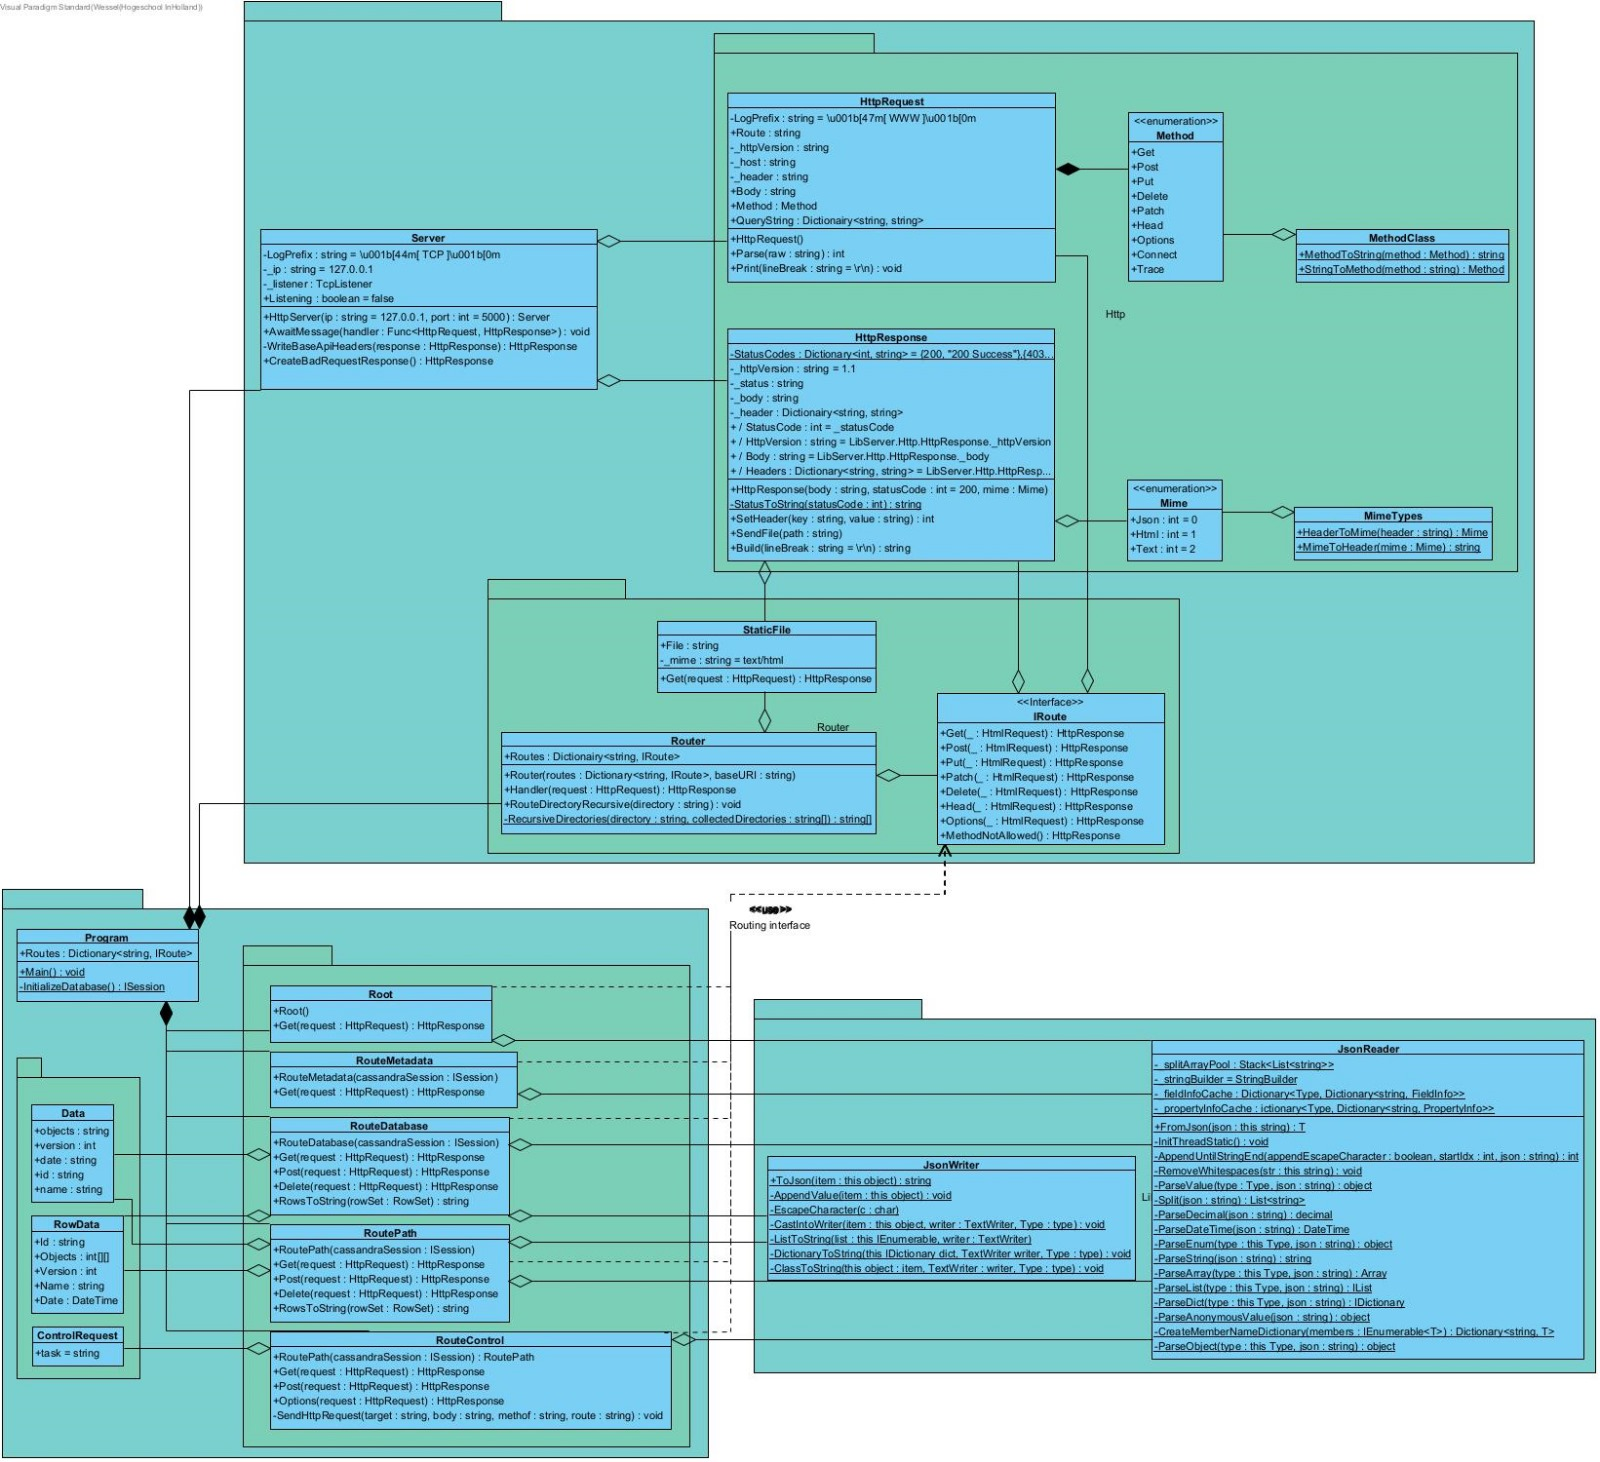
\includegraphics[width=0.5\textwidth]{uml.jpg}
    \caption{Resulterende UML voor de API server.}
    \label{fig:uml}
\end{figure}



\section*{Erkenningen}
\label{sec:erkenningen}
De auteur wilt graag de volgende mensen bedanken voor hun contributie bij het schrijven van dit verslag:
\begin{itemize}
  \item[] \makebox[3.2cm]{\textbf{Buurman, W. J.}\hfill} Groepsgenoot
  \item[] \makebox[3.2cm]{\textbf{Slikker, T.}\hfill} Groepsgenoot
  \item[] \makebox[3.2cm]{\textbf{Ottens, N.}\hfill} Begeleiding
  \item[] \makebox[3.2cm]{\textbf{Tilmann, K.}\hfill} Begeleiding
\end{itemize}

\label{sec:referenties}
\bibliographystyle{IEEEtran}
\bibliography{references}
% \nocite{*}

\end{document}
